\chapter{Implementation}
\section{Input}	% svg files, why vector is better than raster
For the implementation of the presented algorithms an input format had to be specified. As already mentioned in the requirements, it was desired that the input would be easy to edit for artists. That implies that a proper editing tool should be available. To create drawings basically two types of representation are existing: raster images and vector graphics. Raster images work on a \textit{pixel} basis. Each pixel is saved as respective color value depending on the color space (grayscale, indexed or RGB are common). Lossy compression for raster images is available. Scaling raster graphics is limited by the resolution the image was saved in.

In contrast, vector graphics have infinite resolution because they define the image in terms of mathematical functions. Vector graphics contain information about seperate elements where raster graphics do only contain color information and don't have any concept of \enquote{element}. That makes it easy to retrieve and store metadata and, for example, parse the color of a line or area.

Due to the mentioned points it was easy to decide that vector graphics will be used as input for the path generator program. Several excellent editors are existing, such as Inkscape, which was already mentioned in the beginning, or Adobe® Illustrator®, which is a graphics industry standard.

Since vector graphics is only a concept, a file format has to be specified as well. A number of proprietary formats, like the Adobe® Illustrator® format (\texttt{.ai}) are available, but because of their proprietary nature they have been ruled out. The most widely supported format for vector graphics is the \textit{Scalable Vector Graphics} (SVG) specification, which is an open standard format, defined by the SVG Working Group\cite{svgstandard}. Rendering SVG is supported in all major web browsers and most modern user interface toolkits such as QT or GTK+. SVG is based on the \textit{Extended Markup Language} (XML), for which a number of proprietary and open source parsers are available, thus making it easy to build upon.

\section{SVG Parser}

The main part of the SVG specification that we needed to implement is the path parsing. A path, in SVG, is represented by a sequence of commands. A command is a lower- or uppercase letter followed by a list of coordinates
\footnote{\url{http://www.w3.org/TR/SVG/paths.html}}. Coordinates following uppercase letters indicate \textit{absolute} coordinates and lowercase letter are followed by \textit{relative} coordinates. It is stateful in the way that for correct parsing the previous coordinate has to be known, except for the \texttt{M} (Move To) command.

A not complete list of possible commands is listed below:

\begin{description}
\item[\texttt{[M/m] (x,y)+}] Move To command. Starts a new (sub-)path at x,y.
\item[\texttt{[L/l] (x,y)+}] Line To command. Draws a straight line from the previous coordinate to the current coordinate.
\item[\texttt{[C/c] (x1, y1, x2, y2, x3, y3)+}] Curve To command. Defines a cubic Beziér curve with 4 control points.
\item[\texttt{Z}] Closes the element.
\end{description} 

The SVG parser is implemented in Python. After an initial attempt to use an implementation by the author, it reached a certain limit of complexity that was needed to deal with output produced by Inkscape, and a rewrite would have been imminent. The implementation did not regard element-wise transforms nor to inheritance of group transforms, where a parsing tree structure would be needed. Luckily, a good implementation of all necessary features for the path generation was found online, called \enquote{svg} \footnote{\url{https://github.com/cjlano/svg}}.

It was enhanced by an attribute parser and some smaller changes to the inner workings were made to produce the necessary output. The SVG parser also has functions to reduce Beziér splines to a polyline by evaluating the polynomial at certain, linearly distributed intervals of $t \in [0, 1]$. The resulting points are not equally spaced, which is a property of Beziér curves. The points are, however, more densly spaced in regions where the curvature is higher and that is actually positive as the region with the most change gets the most \enquote{attention}. 

A wrapper script was created that exports two functions to the main path generator and passes the parsed objects.	

\section{Element Polymorphism}\label{sec:elem}

An element container class exists from which three different classes are derived (corresponding to the three defined image elements). The classes are \texttt{PolyLineElementPtr}, \texttt{PolygonElementPtr} and \texttt{FilledPolygonElementPtr}.

Some common properties are:

\begin{description}

\item[\texttt{\textcolor{blue}{int} getSize()}] Returns the size of the container holding the vertices.

\item[\texttt{\textcolor{blue}{Point\_2} getFromIndex(\textcolor{blue}{int} idx)}] Returns the point at index. This feature is implemented as circulator by taking the modulo: 
\texttt{return element[idx mod element.size()];}. 
It is useful for accessing the polyon elements as well as the end of a polyline, which can be accessed by calling the
function with \texttt{idx = -1;}.

\item[\texttt{\textcolor{blue}{ElementPtr} * to, from}] see below.
\item[\texttt{\textcolor{blue}{Point\_2} entryPoint, exitPoint}] Those two items keep track of the tour through the drawing. The pointers \texttt{from} and \texttt{to} keep track of the previous and next element. A complete tour is thus saved as a doubly linked list that spans all elements. This structure makes it easy to iterate through the tour.
The \texttt{exitPoint} and \texttt{entryPoint} are the points on the element where the tour is entering and leaving.

\item[\texttt{\textcolor{blue}{TourConnector} enforcedConnection[2]}] An element can have enforced connections to at most two other elements. The tour connector class stores the exit- or entry node (it is not known in which direction a polyline is traversed) as well as the target element.

\item[\vv{int}{enforcedStartIndex}] Stores an optional enforced start index if the traversal of the element should be started at that this index.

\item[\vv{int}{getType();}] returns element type (can be one of \texttt{EL\_POLYLINE}, \texttt{EL\_POLYGON}, \texttt{EL\_FILLED\_POLYGON}, which are defined in a enumeration).

\end{description}

\section{Tree Container}

All elements are sorted into a tree structure. The tree structure was chosen to keep track of the containment information.

\section{Preprocessing}

In the preprocessing phase of the program, the bounding box of all elements is calculated to scale and translate them to the actual canvas size which can be arbitrarily set. An optional margin can be added to the canvas to mitigate the risk of connection lines going outside the canvas and thereby loosing localization or driving into the spectators.

\section{Implementation of the Algorithms}

All core geometric algorithms have been provided by the \textit{Computer Geometric Algorithms Library} (CGAL)\cite{cgal:eb-00a}. CGAL operates with kernels, which implement the common types, such as Point\_2, Line\_2, Segment\_2, Vector\_2, Polygon\_2. Since exact constructions are not necessary for our goals, the 
\enquote{exact predicates inexact constructions kernel} is used throughout the application, which stores all coordinates as double-precision floating-point values (and is thereby limiting the exactness of constructions). The functions that are used the most in this implementation are \texttt{CGAL::intersect}, \texttt{CGAL::transform} and \texttt{CGAL::squared\_distance}. Vector algebra is also simple thanks to operator overloading.

CGAL contains algorithms for the straight skeleton methods\cite{cgal:c-sspo2-14a} as well as for the convex decomposition\cite{cgal:h-pp2-00a}.

\section{Post Processing}

After the complete trajectory for the drawing process was evaluated and, eventually modified, in the graphical user interface, the post processing step does two enhancements.

First, the edges of the trajectory are rounded. The fill elements are receiving an inner rounding, whereas the outer elements (polygon boundaries) are rounded by analysing a threshold angle. If the angle is too sharp, the trajectory will create an outer loop so that the edges will stay sharp (illustrated in \autoref{fig:rounding}. Otherwise, the rounding is also on the inner side. Both inner and outer rounding are created by applying vector math to the problem. For the outer rounding, vectors along both tangents are elongated until the distance between the endpoints fits an arc with radius $r$. While this works for the general case, it shows undesired behaviour for small angles. The tangents have to be very far elongated until the arc fits between, approaching an elongation length of inifinity for a 0 degree angle between the tangents. This behaviour is obviously undesired. Therefore, an implementation based on the spiro connections between elements was thought of but not yet implemented. 

In the next step, all connecting curves are discretized to polylines and the complete trajectory is equally spaced with points and corresponding rake states, so that it can easily be handled by the \textit{Path Converter} or directly be passed to the point following controller of the BeachBot.

\begin{figure}
\centering
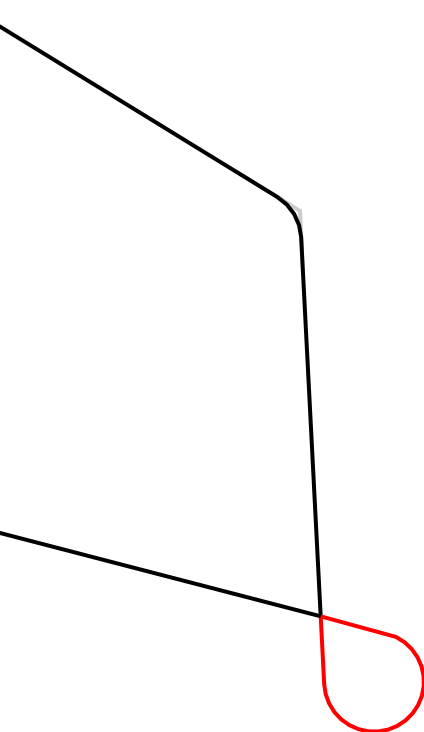
\includegraphics[width=0.5\textwidth]{images/implementation/rounding_edges.pdf}
\caption{Rounding edges either on the inside or the outside.}
\end{figure}

\section{User Interface}

The graphical user interface (GUI), that runs in a regular web browser, was implemented in \textit{JavaScript}, or, more specifically in \textit{CoffeeScript}, which compiles to regular JavaScript. A screenshot of the user interface is shown in \autoref{screenshots}. The \textit{paper.js}\footnote{\url{http://paperjs.org/}} library was used for drawing and provides most of the abstractions used throughout the program. A \textit{Python} server is used as slim host of the main application. The application provides means to parse and send JSON serializations of the complete vector element tree, which are parsed in the JavaScript user interface. All data is sent and retrieved using asynchronous \texttt{GET} and \texttt{POST} requests (commonly referred to as \textit{AJAX}). This implementation was chosen to allow for great flexibility in terms of devices accessing the server. A separate bachelor thesis was working on a Android tablet based touch interface to control the BeachBot. Since Android tablets are perfectly capable of including a \textit{WebView} component which could easily serve the \textit{HTML} and JavaScript files developed in this bachelor thesis, integration of those two tools would be relatively easy. The main program also compiles on the internal computer of the BeachBot, where the server could possibly run, allowing for a fully integrated system. As mentioned in \autoref{sec:elem}, all elements have a unique identifier which makes it easy to select them in the element container and what is used by several of the user interface methods.

Three different view modes and four tools have been implemented which have proven to be helpful in the design of useful trajectories for the BeachBot.

\begin{figure}

\begin{subfigure}[t]{0.45\textwidth}
\includegraphics[width=\textwidth]{images/ui/i1.png}
\caption{The user interface with Outline View activated}\label{fig:outline_view}
\end{subfigure}~
\begin{subfigure}[t]{0.45\textwidth}
\includegraphics[width=\textwidth]{images/ui/i2.png}
\caption{Realistic View activated}\label{fig:real_view}
\end{subfigure}\par \bigskip
\begin{subfigure}[t]{0.45\textwidth}
\includegraphics[width=\textwidth]{images/ui/i3.png}
\caption{Showing connections as arrows}\label{fig:simple_conn}
\end{subfigure}~
\begin{subfigure}[t]{0.45\textwidth}
\includegraphics[width=\textwidth]{images/ui/i4.png}
\caption{Editing the connection curve}
\end{subfigure}~
\caption{Screenshots of the graphical user interface.}\label{screenshots}
\end{figure}

\subsection{Views} The \textit{Outline} view (\autoref{fig:outline_view}) is the standard view, where all paths of the image are displayed with a stroke width of 2 pixels. The \textit{Realistic} view (\autoref{fig:real_view}) tries to approximate the real rake size of the generated trajectory by using a stroke width that corresponds to the real world dimensions. Empirical data shows that the conversion does work reasonably well. The connections can also be displayed differently. If \textit{Show Connections} is selected, all connecting trajectories are rendered in red color on the screen. Selecting \textit{Simple Connection} (\autoref{fig:simple_conn}), the connections are rendered as directed arrows, which is useful for changing and analyzing the TSP solution. \textit{No Connections} hides all the connecting trajectories. All view code is implemented client-side (in JavaScript).
The user can zoom in and out of the drawing by scrolling the mouse-wheel up and down, as well as pan the view by pressing and holding the right mouse button and dragging the cursor across the screen.

\subsection{Tools}

Paper.js offers a useful tool abstraction layer, which makes the creation of various tools very flexible. Four different tools have been implemented:

\begin{description}
\item[Change Connection Tool] As mentioned, the \texttt{ElementPtr} can store enforced connections between elements. Selecting the first or last node of a polyline or any node of a polygon element, and subsequently the same on another element adds an enforced connection between those elements at the desired nodes, and also deletes any previous enforced connection between the node and any other element.
\item[Shape Transitions Tool] The transitions, as they are a set of cubic Beziér curves, sometimes have to be modified because they cross an area or show otherwise undesired behaviour. While for example the crossing of already drawn areas could also be mitigated in the code, it was not possible to do so in the scope of this bachelor thesis. The shape transitions tool offers a convenient way to so: just like in vector graphics programs the node can be selected, which then also displays its two handles. The handles or the node itself can be moved. However, the rotation of the handles (which influences the continuity of the curve), is kept so that both handles form a straight line (the length of the handle vector is not influenced by an operation on the other one).
\item[Select Fill Tool] As discussed, two different fill mechanisms are available: The spiral fill and the back and forth fill. Selecting a convex segment of a partitioned polygon, a vector can be drawn that indictates the desired direction of back-and-forth fill for the selected segment. In the same way, the selected segment can also be chosen to be filled by a spiral by clicking the \textit{Use Spiral Fill} button.
\item[Segmentation Tool] If the segmentation of a polygon is not as desired, the segmentation tool can be used to resegment the polygon. Drawing a line from any point to another sends a segmentation request to the server. If any of the filled polygons is intersecting with the drawn line segment, the polygon will be cutted along it, yielding two or more polygons. Afterwards, the optimal convex partitioning is executed on each of the new segments.
\end{description} 
